% !Mode:: "TeX:UTF-8"


\subsubsection{1.2 国内外研究现状-参考文献说明}
参考文献有两种格式引入\verb+\cite{}+以及\verb+\citep{}+。使用效果可见下面介绍:\\
1.插入会议inproceedings\cite{zhao2015bearing}\\
2.插入教材课本book\cite{williams1991probability,chengzhaolin2006}\\
3.插入期刊article\cite{cao2011formation,xue2015formation},期刊上标\citep{xue2015formation}\\
4.插入硕博论文thesis\cite{lisi2015,wangwu2015,deans2005bearings}\\
5.插入网站misc\cite{irdawebsite,h7n9,wikipedia_moores_law}\\
6.插入专利patent\cite{xiao2012yi,p6915001}\\
7.插入新闻news报纸newspaper\cite{zhang2000,renminribao}\\
8.插入标准standard\cite{gbt3469-1983}\\
\textcolor{red}{注意:参考文献格式不正确可能导致编译不通过,大家可以参考本工程中reference.bib中文献格式对网上下载不规范的bibtex文件进行修改。此外,如果上述类型里面条目有缺失会会导致编译不能输出正确格式。}关于参考文献不同类型的进一步详细的说明可参考网站https://github.com/Haixing-Hu/GBT7714-2005-BibTeX-Style
里面的测试模板。

\textcolor{red}{注意1:参考文献格式不正确可能导致编译不通过,大家可以参考本工程中reference.bib中文献格式对网上下载不规范的bibtex文件进行修改。此外,如果上述类型里面条目有缺失会会导致编译不能输出正确格式。}

关于参考文献不同类型的进一步详细的说明可参考网站https://github.com/Haixing-Hu/GBT7714-2005-BibTeX-Style
里面的测试模板。


\textcolor{red}{注意2:对于中文参考文献,为了保证格式正确,最好需在对应bib里面添加language={zh},不加会默认当做英文文献处理。区别如图\ref{fig_bib0}。}

\begin{figure}[!htb]
  \centering
  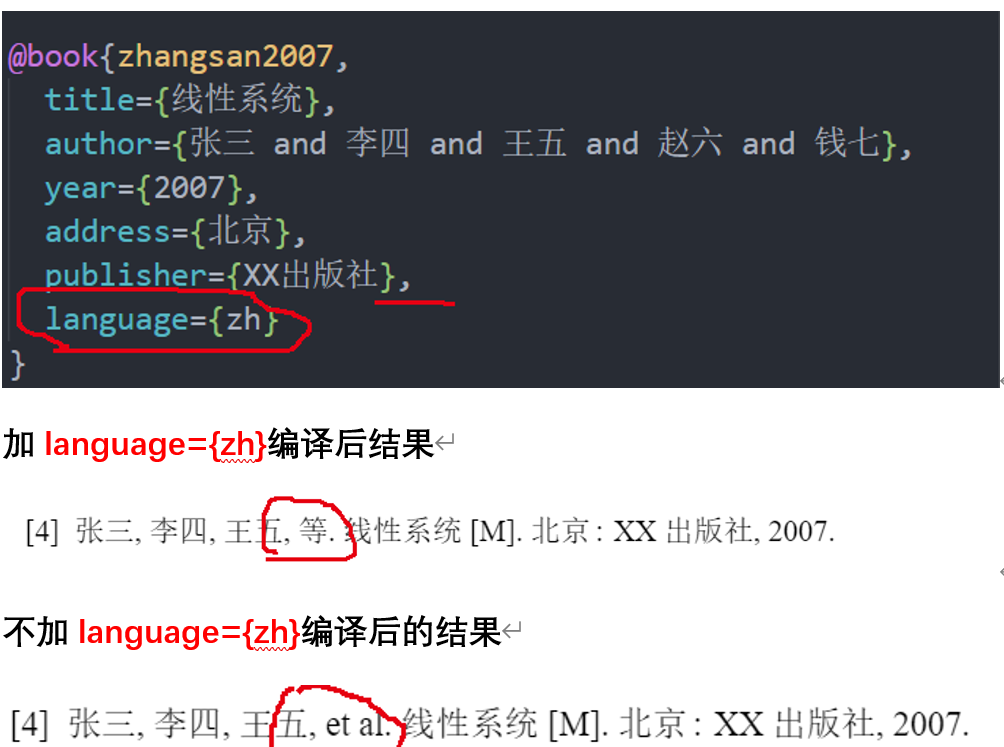
\includegraphics[width=1\textwidth]{中英文文献bib编译注意事项}
  \caption{中英文文献bib编译注意事项以作者超过3个为例进行说明}
  \label{fig_bib0}
\end{figure}




